
\definecolor{dkgreen}{rgb}{0,0.6,0}
\definecolor{gray}{rgb}{0.5,0.5,0.5}
\definecolor{mauve}{rgb}{0.58,0,0.82}
\lstset{frame=tb,
  language=Java,
  aboveskip=3mm,
  belowskip=3mm,
  showstringspaces=false,
  columns=flexible,
  basicstyle={\small\ttfamily},
  numbers=none,
  numberstyle=\tiny\color{gray},
  keywordstyle=\color{blue},
  commentstyle=\color{dkgreen},
  stringstyle=\color{mauve},
  breaklines=true,
  breakatwhitespace=true,
  tabsize=3
}

\section{Kamehameha}

\subsection{Descripción del problema}

El problema consiste en calcular la mínima cantidad de Kamehamehas que debe lanzar Goku para destruir un conjunto de andriodes usando Backtracking.
Al usar backtracking, el problema se reduce a trazar todas las posibles rectas que pasan una sola vez por cada punto y elegir la combinación con menor cantidad de rectas. En el siguiente gráfico se muestra un ejemplo con 5 androides en las siguientes posiciones
1 (1,2) 2 (2,1) 3 (3,2) 4 (4,2) 5 (3,3)
\begin{figure}[h!]
  \centering
  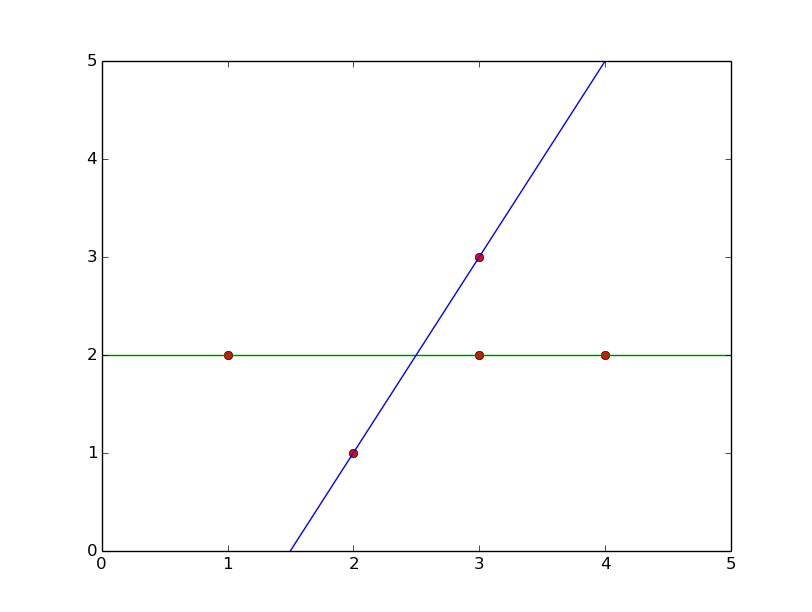
\includegraphics[width=7cm, height=6cm]{ejemploHame1}
  \caption{Solución para un caso con 5 androides.}
\end{figure}

Una posible solución óptima sería lanzar dos Kamehameha, uno que mate a 3 androides (al 1, 3 y 4), la recta verde, y otro que mate a los otros 2, la recta azul. En este caso la solución es única.

\subsection{Descripción de la resolución}
La idea del algoritmo es que recursivamente vaya creando todas las combinaciones de rectas. Esto lo logramos utilizando una función principal a la que llamamos recursivamente, Kamehameha,  y dos funciones, una que se fija si un androide puede ser atacado con un Kamehameha ya lanzado (si está alineado con algún otro grupo de androides ya atacados) y vuelve a llamar a la función principal con los nuevos valores una vez por cada grupo con el que está alineado este androide; y otra función que comienza un nuevo ataque con ese androide y vuelve a llamar a la función principal.
\par{De esta forma, probando con un enemigo, volviendo atrás, probando con el siguiente, volviendo atrás y así sucesivamente hasta probar con todos los enemigos, podemos generar todas las posibles combinaciones de líneas. Lo único que resta es verificar cuál de estas es la óptima. Para conseguirlo, cada vez que generamos una solución completa, verificamos su tamaño (su cantidad de líneas) y la guardamos si es la menor hasta el momento, si no la descartamos.}
\par{Para mejorar el tiempo de ejecución decidimos agregar una poda que descarta soluciones que están siendo generadas en el momento que su tamaño supera el tamaño de la solución mínima alamacenada, ya que sabemos que es mayor o igual a la que ya tenemos y por lo tanto no nos sirve.}

\subsection{Cota de complejidad}
Como la cantidad de posibles combinaciones distitnas de $n$ andoides con $n$ androides distintos es análoga a la cantidad de números de $n$ digitos distintos que se pueden armar con $n$ números de un digito distintos, ya que el primer androide que tomemos, lo podemos dejar solo o juntarlo con cualquiera de los otros $n-1$ androides lo que le da $n$ posibles opciones. Una vez que el primero esta fijo, hacemos lo mismo con el segundo androide, puede quedarse donde está o juntarse con cualquiera de los otros $n-2$ androides que aún no tienen posición fija, lo que le da $n-1$ posibilidades. Luego hacemos lo mismo con el resto de los androides, cada uno tendra la cantidad de posibilidades que tenía el androide anterior $-1$, hasta llegar al último androide que queda con 1 sola posibilidad, quedarse dodne está. Así se puede ver que la cantidad todal de combinasciones es $n*(n-1)*(n-2)*...*(n-(n+2))*(n-(n+1))$ que da $n!$.
Por lo tanto, la cantidad de hojas de nuestro árbol de recursión, es decir la cantidad de soluciones posibles, como no se llega a la misma solución más de una vez, está acotada por $n!$.

Por cómo planteamos la resolución del problema, por cada solución que generamos, volvemos atrás y reutilizamos lo ya calculado para generar todas las posibles. De esta forma las hojas de nuestro árbol tienen siempre al menos un hermano. Suponiendo el peor caso, donde cada hoja tiene solamente un hermano, como cada sub solución es una solución posible de un problema de menor tamaño, podemos asumir que todo nodo tiene solamente un hermano, convirtiendo a nuestro árbol de recursión en un árbol binario. Teniendo $n!$ hojas y siendo la cantidad total de nodos $= (($\#$hojas)*2 - 1)$ nos da que la cantidad de nodos es del orden de $2*n!$ por lo tanto la complejidad del algoritmo termina siendo $\mathcal{O}(n!)$.

Teniendo en cuenta las podas el mejor caso ocurre cuando están todos los androides alineados ya que al comparar el tamaño de las soluciones se descartan todas las que tienen más que un Kamehameha. Por otro lado, el peor caso se da cuando no hay más de 2 androides para una misma recta debido a que las soluciones en su mayoría van a tener la misma cantidad de rectas.

\subsection{Pseudocódigo}
listaPos $= lista<(int,int)>$ , kamehamehas $= lista<(listaPos)>$

\begin{algorithm}
\caption{Kamehameha}
\begin{algorithmic}
  \Function{Kamehameha}{$enemigos$: listaPos, $ataques$: Kamehamehas, $nroAtaque$: int} 
	\If{$minimoGlobal$ $\leq$ size($ataques$)} \Comment $\mathcal{O}(1)$
		\State return \Comment $\mathcal{O}(1)$
	\EndIf
	\If{size($enemigos$) $=$ $0$)} \Comment $\mathcal{O}(1)$
		\If{$minimoGlobal$ $>$ size($ataques$)}\Comment $\mathcal{O}(1)$
			\State $minimoGlobal \gets$ size($ataques$) \Comment $\mathcal{O}(1)$ 		
			\State $mejorConfiguracion \gets ataques$ \Comment $\mathcal{O}(1)$
		\EndIf
	\Else
		\State $enemigo \gets enemigos[0]$ \Comment $\mathcal{O}(1)$
		\State erase($enemigo$, $enemigos$) \Comment $\mathcal{O}($size($enemigos$))
		\State AtacarEnAtacados($enemigo$, $enemigos$, $ataques$, $nroAtaques$)	\Comment $\mathcal{O}(nroAtaques)$
		\State AtacarEnNuevoAtaque($enemigo$, $enemigos$, $ataques$, $nroAtaques$) \Comment $\mathcal{O}(1)$
		\State insert($enemigo$, $enemigos$) \Comment $\mathcal{O}($size($enemigos$))
\EndIf
\EndFunction
\end{algorithmic}
\underline{Complejidad:} $\mathcal{O}(n!)$\\
    
\end{algorithm}

\begin{algorithm}
\caption{AtacarEnAtacados}
\begin{algorithmic}
  \Function{AtacarEnAtacados}{$enemigo$: posición, $restoEnemigos$: listaPos, $ataques$: Kamehamehas, $nroAtaques$: int}
\State $i \gets 0$ \Comment $\mathcal{O}(1)$
\State $atacados \gets nuevaListaPos()$ \Comment $\mathcal{O}(1)$
\While{$i \leq nroAtaques$} \Comment $\mathcal{O}(nroAtaques)$
	\State $atacados \gets ataques[i]$ \Comment $\mathcal{O}(1)$
	\If{size($atacados$) $=$ $0$} \Comment $\mathcal{O}(1)$
		\State $comenzarAtaque \gets $nuevaListaPos() \Comment $\mathcal{O}(1)$
		\State pushBack($enemigo, comenzarAtaque$) \Comment $\mathcal{O}(1)$
		\State $ataque[i] \gets 	comenzarAtaque$ \Comment $\mathcal{O}(1)$
		\State Kamehameha($restoEnemigos$, $ataques$, $nroAtaques$) \Comment $\mathcal{O}(1)$
		\State $restablecerAtaque \gets $nuevaListaPos() \Comment $\mathcal{O}(1)$
		\State $ataque[i] \gets 	restablecerAtaque$ \Comment $\mathcal{O}(1)$
	\ElsIf{Alineados($atacados$, $enemigo$)} \Comment $\mathcal{O}(1)$
		\State pushBack($enemigo$, $ataque[i]$) \Comment $\mathcal{O}(1)$
		\State Kamehameha($restoEnemigos$, $ataques$, $nroAtaques$) \Comment $\mathcal{O}(1)$
		\State popBack($ataque[i]$) \Comment $\mathcal{O}(1)$
	\EndIf
	\State $i \gets i + 1$ \Comment $\mathcal{O}(1)$
\EndWhile
\EndFunction
\end{algorithmic}
\underline{Complejidad:} $\mathcal{O}(nroAtaques)$\\
    
\end{algorithm}
 \newpage

\begin{algorithm}
\caption{AtacarEnNuevoAtaque}
\begin{algorithmic}
  \Function{AtacarEnNuevoAtaque}{$enemigo$: posicion, $restoEnemigos$: listaPos, $ataques$: Kamehamehas, $nroAtaque$: int}

\If{size($ataque[nroAtaque]$) $>$ $0$} \Comment $\mathcal{O}(1)$
	\State $comenzarAtaque \gets $nuevaListaPos() \Comment $\mathcal{O}(1)$
	\State pushBack($enemigo, comenzarAtque$) \Comment $\mathcal{O}(1)$
	\State pushBack($comenzarAtaque, ataques$) \Comment $\mathcal{O}(1)$
	\State $nroAtaque \gets nroAtaque + 1$ \Comment $\mathcal{O}(1)$
	\State Kamehameha($restoEnemigos$, $ataques$, $nroAtaques$) \Comment $\mathcal{O}(1)$
	\State $nroAtaque \gets 	nroAtaque - 1$ \Comment $\mathcal{O}(1)$
	\State popBack($ataque$) \Comment $\mathcal{O}(1)$
\EndIf

\EndFunction
\end{algorithmic}
\underline{Complejidad:} $\mathcal{O}(1)$\\
\end{algorithm}

\begin{algorithm}
\caption{Alineados}
\begin{algorithmic}
  \Function{Alineados}{$atacados$: kamehameha, $enemigo$: posicion}{Bool} 
  	\If{size($atacados$) $\leq$ $1$} \Comment $\mathcal{O}(1)$
  		\State return $true$ \Comment $\mathcal{O}(1)$
  	\Else
  		\State $primero \gets atacados[0]$ \Comment $\mathcal{O}(1)$
  		\State $segundo \gets atacados[1]$ \Comment $\mathcal{O}(1)$
  		\State $termino1 \gets segundo[1] - primero[1]$ \Comment $\mathcal{O}(1)$
  		\State $termino2 \gets enemigo[0] - primero[0]$ \Comment $\mathcal{O}(1)$
    		\State $termino3 \gets enemigo[1] - primero[1]$ \Comment $\mathcal{O}(1)$
      	\State $termino4 \gets segundo[0] - primero[0]$ \Comment $\mathcal{O}(1)$
      	\State return $termino1*termino2 = termino3*termino4$ \Comment $\mathcal{O}(1)$ 
  	\EndIf
\EndFunction
\end{algorithmic}
\underline{Complejidad:} $\mathcal{O}(1)$\\
\end{algorithm}


\subsection{Experimentación}
Experimentando con el algoritmo nos dimos cuenta de que el tiempo de ejecución variaba un poco dependiendo del momento particular en que se corriera el programa, de la distribución de los puntos o del funcionamiento de la máquina. Es por esto que decidimos ejecutarlo 5 veces para cada grupo de n puntos y tomar al promedio de los mismos como una referencia más confiable. Lo hicimos con $n=1$ a $10$. 
\par{A continuación se exponen la tabla y el gráfico resultante de esas mediciones}
\\
\begin{table}[h]
\centering
\label{my-label}
\begin{tabular}{cc}
\hline
\multicolumn{1}{|c|}{n (Tamaño de la entrada)} & \multicolumn{1}{c|}{Tiempo (segundos)} \\ \hline
\multicolumn{1}{|c|}{1}                        & \multicolumn{1}{c|}{$2.78 \times 10^{-5}$}         \\ \hline
\multicolumn{1}{|c|}{2}                        & \multicolumn{1}{c|}{$3.02 \times 10^{-5}$}            \\ \hline
\multicolumn{1}{|c|}{3}                        & \multicolumn{1}{c|}{$4.30 \times 10^{-5}$}               \\ \hline
\multicolumn{1}{|c|}{4}                        & \multicolumn{1}{c|}{$5.54 \times 10^{-5}$}            \\ \hline
\multicolumn{1}{|c|}{5}                        & \multicolumn{1}{c|}               {$1.43 \times 10^{-4}$}  \\ \hline
\multicolumn{1}{|c|}{6}                        & \multicolumn{1}{c|}                  {$1.58 \times 10^{-4}$}  \\ \hline
\multicolumn{1}{|c|}{7}                        & \multicolumn{1}{c|}                  {$6.88 \times 10^{-4}$}  \\ \hline
\multicolumn{1}{|c|}{8}                        & \multicolumn{1}{c|}                  {$9.09 \times 10^{-4}$}  \\ \hline
\multicolumn{1}{|c|}{9}                        & \multicolumn{1}{c|}                  {$3.31 \times 10^{-3}$}  \\ \hline
\multicolumn{1}{|c|}{10}                        & \multicolumn{1}{c|}                  {$4.38 \times 10^{-3}$}  \\ \hline

\end{tabular}
\caption{Tabla que muestra los tiempos de ejecución correspondientes a distintos tamaños de entrada.}
\end{table}

\begin{figure}[h!]
  \centering
  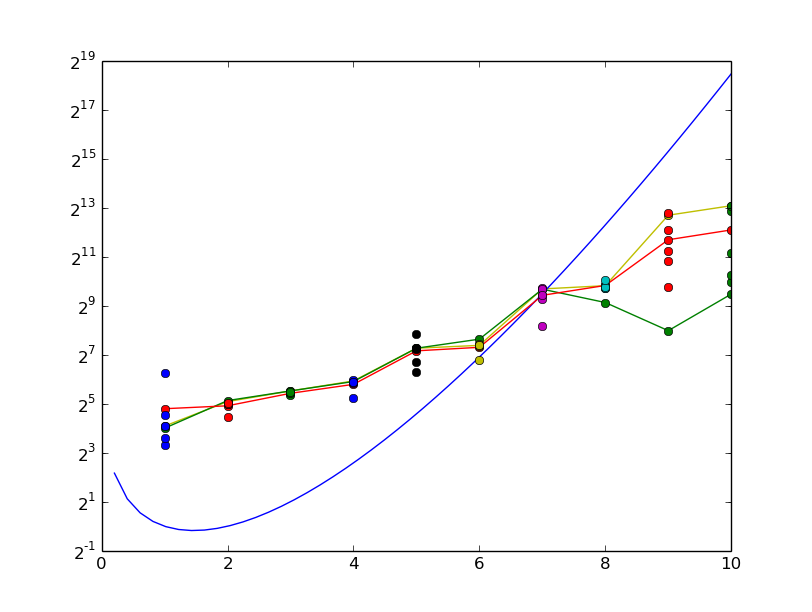
\includegraphics[width=12cm, height=9cm]{HameTime}
  \caption{Tiempos de ejecución para distintas entradas. La curva azul es la curva de la complejidad, $n!$, la línea verde es mejor caso, la roja caso aleatorio y la amarilla peor caso.}
\end{figure}

\newpage
\subsection{Apéndice: código de Genkidama}
\begin{lstlisting}

#include <iostream>
#include <deque>
#include <utility>
#include <vector>
#include <stdlib.h>
#include <time.h>
#include <algorithm>
#include <limits>
using namespace std;

typedef pair<int,int> posicion_t;
typedef vector<posicion_t> Kamehameha_t;
typedef vector<Kamehameha_t> Kamehamehas_t;
typedef deque<posicion_t> listaPos_t;

int minimo_global = std::numeric_limits<int>::max();
listaPos_t enemigos_global;
Kamehamehas_t mejor_configuracion;

void Kamehameha(listaPos_t enemigos,
                Kamehamehas_t enLaMira,
                int indexRectaActual);
void atacarEnAtaqueActual(posicion_t enemigo,
                          listaPos_t restoEnemigos,
                          Kamehamehas_t ataques,
                          int nroAtaque);
void atacarEnNuevoAtaque(posicion_t enemigo,
                         listaPos_t restoEnemigos,
                         Kamehamehas_t ataques,
                         int nroAtaque);
bool alineados (Kamehameha_t atacados, posicion_t enemigo);
void reporte(listaPos_t enemigos, Kamehamehas_t ataques, int nroAtaque);
int buscarPosicion(const posicion_t& enemigo);
void mostrarSolucion();

int main() {
    int cantEnemigos;
    cin >> cantEnemigos;
    listaPos_t enemigos;
    Kamehamehas_t enLaMira;
    Kamehameha_t kamehameha;
    enLaMira.push_back(kamehameha);
    int indexRectaActual;
    posicion_t posicion;

    for (int i = 0; i < cantEnemigos; i++) {
        int x;
        int y;
        cin >> x >> y;
    	posicion = make_pair(x, y);
    	enemigos.push_back((posicion));
    }

    enemigos_global = enemigos;
    for (listaPos_t::iterator it = enemigos.begin(); it != enemigos.end(); ++it) {
            cerr << (*it).first << " " << (*it).second << endl;
    }
    Kamehameha(enemigos, enLaMira, 0);
    mostrarSolucion();
    return 0;
}

void Kamehameha(listaPos_t enemigos, Kamehamehas_t ataques, int nroAtaque) {
    if (minimo_global <= (int) ataques.size()) {
      return;
    }
    if (enemigos.size() == 0) {
        if (minimo_global > (int) ataques.size()) {
            minimo_global = (int) ataques.size();
            mejor_configuracion = ataques;
        }
    } else {
        for (int i = 0; i < enemigos.size(); i++) {
            posicion_t const enemigo = enemigos[i];
            enemigos.erase(enemigos.begin()+i);
            atacarEnAtaqueActual(enemigo, enemigos, ataques, nroAtaque);
            atacarEnNuevoAtaque(enemigo, enemigos, ataques, nroAtaque);
            listaPos_t::iterator it = enemigos.insert(enemigos.begin()+i, enemigo);
        }
    }
}

void atacarEnAtaqueActual(posicion_t enemigo, listaPos_t restoEnemigos, Kamehamehas_t ataques, int nroAtaque) {
    Kamehameha_t atacados = ataques[nroAtaque];
    if (atacados.size() == 0){
        Kamehameha_t comenzarAtaque;
        comenzarAtaque.push_back(enemigo);
        ataques[nroAtaque] = comenzarAtaque;
        Kamehameha(restoEnemigos, ataques, nroAtaque);
        Kamehameha_t reestablecerAtaque;
        ataques[nroAtaque] = reestablecerAtaque;
    } else if (alineados(atacados, enemigo)) {
        ataques[nroAtaque].push_back(enemigo);
        Kamehameha(restoEnemigos, ataques, nroAtaque);
        ataques[nroAtaque].pop_back();
    } else {
        return;
    }
}

void atacarEnNuevoAtaque(posicion_t enemigo, listaPos_t restoEnemigos, Kamehamehas_t ataques, int nroAtaque) {
    if (ataques[nroAtaque].size() > 0) {
        Kamehameha_t comenzarAtaque;
        comenzarAtaque.push_back(enemigo);
        ataques.push_back(comenzarAtaque);
        nroAtaque++;
        Kamehameha(restoEnemigos, ataques, nroAtaque);
        nroAtaque--;
        ataques.pop_back();
    }
}

bool alineados (Kamehameha_t atacados, posicion_t enemigo) {
    if (atacados.size() == 0 || atacados.size() == 1) {
        return true;
    } else {
        posicion_t primero = atacados[0];
        posicion_t segundo = atacados[1];
        int termino1 = segundo.second - primero.second;
        int termino2 = enemigo.first - primero.first;
        int termino3 = enemigo.second - primero.second;
        int termino4 = segundo.first - primero.first;
        return termino1*termino2 == termino3*termino4;
    }
}

void reporte(listaPos_t enemigos, Kamehamehas_t ataques, int nroAtaque) {
    cout << "enemigos: ";
    for (listaPos_t::iterator itL = enemigos.begin(); itL != enemigos.end(); ++itL) {
        cout << "(" << (*itL).first << ", " << (*itL).second << ")";
        if (itL!= enemigos.end()) {
            cout << ", ";
        }
    }
    cout << endl ;
    for (int i = 0; i < ataques.size(); i++) {
        Kamehameha_t ataqueEnIdx = ataques[i];
        cout << "[";
        for (Kamehameha_t::iterator it = ataqueEnIdx.begin(); it != ataqueEnIdx.end(); ++it) {
            cout << "(" << (*it).first << ", " << (*it).second << "), ";
            if (it!= ataqueEnIdx.end()){ cout << ", "; };
        }
        cout << "]" << endl;
    }
}

void mostrarSolucion() {
    cout << mejor_configuracion.size() << endl;
    for (int i = 0; i < mejor_configuracion.size(); i++) {
        Kamehameha_t ataqueEnIdx = mejor_configuracion[i];
        cout << ataqueEnIdx.size() << " ";
        for (Kamehameha_t::iterator it = ataqueEnIdx.begin(); it != ataqueEnIdx.end(); ++it) {
            cout << buscarPosicion(*it)+1 << " ";
        }
        cout << endl;
    }
}

int buscarPosicion(const posicion_t& enemigo) {
    listaPos_t::iterator it = find (enemigos_global.begin(), enemigos_global.end(), enemigo);
    return distance(enemigos_global.begin(), it);
}
\end{lstlisting}